
\begin{frame}
\frametitle{Binary Search}
\textbf{Binary Search} - a classical strategy used to efficiently locate a hidden target element $t$ in a linearly ordered set $S$ using $O\br{\log n}$ comparison operations.
\pause

\begin{figure}[ht]
\centering
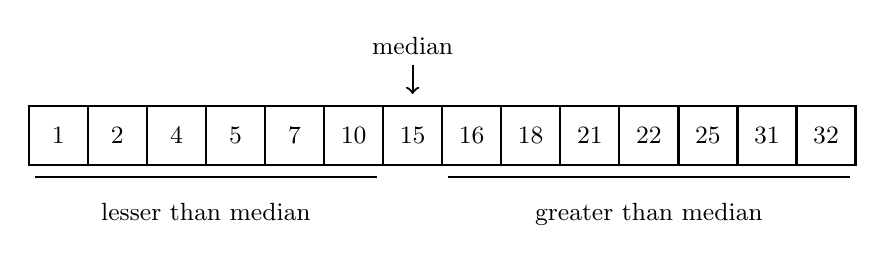
\begin{tikzpicture}[every node/.style={font=\small}, scale=0.75]

% --- Array values (10 elements) ---
\def\A{{1, 2, 4, 5, 7, 10, 15, 16, 18, 21, 22, 25, 31, 32}}
\def\MID{6} % Index of median (0-based): value = 23
% Draw array elements and indices
\foreach \i in {0,...,13} {
    \pgfmathsetmacro{\val}{\A[\i]}
    \draw[thick] (\i, 0) rectangle ++(1,1);
    \node at (\i+0.5, 0.5) {\val};
}

% Underline LEFT subarray (0..3)
\draw[thick] (0.1, -0.2) -- (6.0-0.1, -0.2);
% Label
\node[below=6pt] at (3, -0.2) {lesser than median};

% Underline RIGHT subarray (5..9)
\draw[thick] (7+0.1, -0.2) -- (13+1-0.1, -0.2);
% Label
\node[below=6pt] at (10.5, -0.2) {greater than median};

% Arrow for mid
\draw[<-, thick] (\MID+0.5, 1.2) -- +(0, 0.5) node[above] {median};

\end{tikzpicture}
\caption[Binary search]{Example of a sorted array containing 14 elements. }
\label{fig:binary-search-subarrays}
\end{figure}


\end{frame}

\begin{frame}
\frametitle{Searching in Graphs}
Easy to generalize to trees: A \textbf{query} to a vertex $v$ returns information whether $v$ is the target, and if not, which connected component of $G-v$ contains $t$. The question is: 

\textbf{What is the best strategy of searching in a graph?}
\pause

\begin{figure}[htbp]
    \centering
    \begin{minipage}{0.32\textwidth}
        \centering
        \tikz [node distance = 16mm, rotate=-90]
        \graph [spring layout]
{
  a -- { b, c, d, e};
  b -- {c};
  e -- {j, h};
  d -- {i, f};
  j -- {g[> orient=right]};
  i -- {j, e, k};
  g -- {l};
  h --  a;
  l -- {k};
};
        \caption[Sample graph and decision tree]{}
        \label{fig:graph}
    \end{minipage}
    \begin{minipage}{0.34\textwidth}
        \centering
        \tikz [tree layout, grow=-90,
               sibling distance=11mm, level distance=14.5mm,]
          \graph {
            ""[as=$e$] ->
            ""[as=$i$] -> { ""[as=$a$] -> { ""[as=$c$] -> ""[as=$b$],  ""[as=$h$],""[as=$f$] -> ""[as=$d$]}, ""[as=$g$] -> {""[as=$j$], ""[as=$k$] -> ""[as=$l$]}}
          };
        \caption[Vertex decision tree for a graph]{}
        \label{fig:dt_g_v}
    \end{minipage}
    \hfill
    \begin{minipage}{0.32\textwidth}
        \centering
        \tikz [tree layout, grow=-90,
               sibling distance=10, 
               level distance=8mm]
            \graph {
            ""[as=$ef$] -> 
            ""[as=$ei$] -> 
            ""[as=$ad$] -> {
                ""[as=$ae$] -> ""[as=$ac$] -> ""[as=$ah$] -> {""[as=$eh$], ""[as=$ab$] -> ""[as=$bc$]},
                ""[as=$ij$] -> ""[as=$ik$] -> {""[as=$di$] -> ""[as=$df$], ""[as=$kl$] -> ""[as=$gl$] -> ""[as=$gj$]}
              }
            };
    \caption[Edge decision tree for a graph]{}
    \label{fig:dt_g_e}
    \end{minipage}
        \caption[Graph and decision trees for it]{Sample input graph $G$ (Figure \ref{fig:graph}) and two decision trees for $G$: one for the Vertex Tree Graph Problem (Figure \ref{fig:dt_g_v}) and one for the Edge Graph Search Problem (Figure \ref{fig:dt_g_e}).}                  \label{fig:sample_decision_trees_for_graph}
\end{figure}

\end{frame}

\begin{frame}
\frametitle{Our setup}
We consider the following variant of this problem:
\begin{tcolorbox}[colback=white, title=Graph Search Problem (GSP), fonttitle=\bfseries, breakable]
\textbf{Input:} Tree $G$, a query cost function $c:V\br{G}\to \mathbb{N}$ and a weight function $w:V\br{G}\to \mathbb{N}$.

\pause
\textbf{Output:} A decision tree $D$ minimizing the weighted average search cost: 
$$c_G\br{D} = \sum_{x\in V\br{G}}w\br{x}\cdot \sum_{q\in Q_G\br{D, x}}c\br{q}.$$
where $Q_G\br{D,x}$ denotes the sequence of queries performed 
along the unique path in $D$ from the root $r\br{D}$ to $x$.
\end{tcolorbox}
\end{frame}

\begin{frame}{Why do we care?}
    Useful in:
    \begin{enumerate}
        \item Scheduling of parallel database join operations,
        \item Automated bug detection in computer code,
        \item Parallel Cholesky factorization of matrices,
        \item Hierarchical clustering of data,
        \item Parallel assembly of multi-part products from their components.
    \end{enumerate}
\end{frame}

\begin{frame}{Why do we care?}
Our setup:
\begin{enumerate}
    \item Average case - it is natural to assume that the search strategies we design are intended to be used repeatedly. 
    \item Weight function - some vertices may serve 
as targets more frequently than the others. 
    \item Query costs - performing a query may require 
significant resources, such as time or money. 
\item Have not yet been investigated.
\end{enumerate} 
\end{frame}

\begin{frame}{Many names}
\begin{itemize}
    \item Binary Search \cite{OnakParys2006GenOfBSSInTsAndFLikePosets,dereniowski2017ApproxSsForGeneralBSinWTs,Deligkas2019BsInGsRev,Emamjomeh2016DetAndProbBSinGs,dereniowski2022CFApproxAlgForBSInTsWithMonoQTimes,dereniowski2024SInTsMonoQTs,noisyBSSFC,Dereniowski2024OnMG,EfficientNoisyBinarySearch,Dereniowski2023Edge},
    \item Tree Search Problem \cite{Jacobs2010OnTheComplexSearchInTsAvg,Cicalese2014ImprovedApproxAvgTs,Cicalese2016OnTSPwNonUniCost}, 
    \item Binary Identification Problem \cite{Cicalese2012BinIdentPForWTs}, 
    \item Ranking Colorings \cite{Knuth1973,Dereniowski2009ERankOfWTs,DereniowskiERAndSInPOSets,DereniowskiEfPQProcByGRank,DereniowskiVxRankOfChGsAndWTs,Lam1998ERankOfGsIsH}, 
    \item Ordered Colorings \cite{KATCHALSKI1995141}, 
    \item Elimination Trees \cite{Pothen1988OptimalEliminationTrees}, 
    \item Hub Labeling \cite{Angelidakis2018ShortestPQ},
    \item Tree-Depth \cite{NESETRIL20061022,BOROWIECKI2023113682},
    \item Partition Trees \cite{Hgemo2024TightAB},
    \item Hierarchical Clustering \cite{Acostfunctionforsimilaritybasedhierarchicalclustering,HCObjFsandAlgs,Approximatehierarchicalclusteringviasparsestcutandspreadingmetrics}, 
    \item Search Trees on Trees \cite{SplayTonT,Fast_app_centroid_trees}, 
    \item LIFO-Search \cite{GIANNOPOULOU20122089}. 
\end{itemize}
\end{frame}

\begin{frame}
\frametitle{How to tackle the problem}
\textbf{Bad news:}
The Graph Search Problem is \textbf{NP-hard} even when restricted to bounded degree trees and bounded diameter diamter trees. 
\pause

We want to find an algorithm providing a good \textbf{approximation} for the problem:
\begin{itemize}
    \item $\br{4+\epsilon}$-approximation for trees.
    \item $O\br{\sqrt{\log n}}$-approximation for general graphs.
\end{itemize}
\end{frame}

\begin{frame}
\frametitle{Weighted $\alpha$-Separator Problem}
\begin{tcolorbox}[colback=white, title=Weighted $\alpha$-Separator Problem, fonttitle=\bfseries, breakable]
\textbf{Input:} Graph $G$, a cost function $c:V\to \mathbb{N}$, a weight function $w:V\to \mathbb{N}$ and a real number $\alpha$.

\pause
\textbf{Output:} A set $S\subseteq V\br{G}$ called \textbf{separator} such that for every $H\in G-S$: $w\br{H}\leq w\br{G}/\alpha$ and $c\br{S}$ is minimized.
\end{tcolorbox}

\end{frame}

\begin{frame}{Example of a separator}
    
\begin{figure}[htbp]
    \centering
    \begin{minipage}{0.65\textwidth}
        \centering
        \tikz [tree layout, grow=-65,
               sibling distance=11mm, level distance=13mm, scale = 0.9, thick]
          \graph {
    ""[as=$a$, draw=red, circle, thick] -- {
        ""[as=$b$] -- ""[as=$c$] -- {
            ""[as=$d$, draw=red, circle, thick] -- ""[as=$e$],
            ""[as=$f$] -- { ""[as=$g$, draw=red, circle, thick], ""[as=$h$], ""[as=$i$] }
        },
        ""[as=$j$, draw=red, circle, thick] -- ""[as=$k$] -- { ""[as=$l$], ""[as=$m$] }
    }
};
    \end{minipage}
    \begin{minipage}{0.3\textwidth}
        \centering
        \footnotesize
        \begin{tabular}{|c|c|c|}
\hline
 & $w\br{v}$ & $c\br{v}$\\
\hline
$a$ & 2 & 3\\
\hline
$b$ & 1 & 4\\
\hline
$c$ & 3 & 6\\
\hline
$d$ & 2 & 2\\
\hline
$e$ & 4 & 1\\
\hline
$f$ & 0 & 3\\
\hline
$g$ & 1 & 1\\
\hline
$h$ & 4 & 3\\
\hline
$i$ & 2 & 3\\
\hline
$j$ & 5 & 2\\
\hline
$k$ & 1 & 2\\
\hline
$l$ & 2 & 3\\
\hline
$m$ & 3 & 4\\
\hline
\end{tabular}
    \end{minipage}
        \caption[Tree and decision trees for it]{Sample input tree $T$ and a weighted $3$-separator (the circled vertices) of cost $8$.}
\end{figure}

\end{frame}

\begin{frame}{How to find the separator}
\textbf{Bad news again}: The Weighted $\alpha$-separator Problem is \textbf{NP-hard} as well, but there exists a biciriteria \textbf{FPTAS} for trees:
\pause
\begin{theorem}
    Let $S$ be an optimal weighted $\alpha$-separator for $\br{T,c,w,\alpha}$. For any $\delta>0$ there exists an algorithm \FSeparatorFPTAS, which returns a separator $S'$, such that:
    \begin{enumerate}
        \item $c\br{S'}\leq c\br{S}$.
        \item $w\br{H}\leq \frac{\br{1+\delta}\cdot w\br{T}}{\alpha}$ for every $H\in T-S'$.
        \item The algorithm runs in $O\br{n^3/\delta^2}$ time.
    \end{enumerate}
\end{theorem}

\end{frame}

\begin{frame}{Min-Ratio Vertex Cut Problem}

\begin{tcolorbox}[colback=white, title= Min-Ratio Vertex Cut Problem, fonttitle=\bfseries, breakable]
\textbf{Input:} Graph $G=\br{V\br{G}, E\br{G}}$, the cost function $c:V\to \mathbb{N}$ and the weight function $w:V\to \mathbb{N}$.

\pause
\textbf{Output:} A partition $\br{A,S,B}$ of $V\br{G}$ called \textit{vertex-cut}, such that there are no $u\in A$ and $v\in B$ for which $uv\in E\br{G}$, minimizing the ratio:
$$
\alpha_{c,w}\br{A,S,B}=\frac{c\br{S}}{w\br{A\cup S}\cdot w\br{B\cup S}}.
$$
\end{tcolorbox}
\end{frame}

\begin{frame}{How to find the cut}
Min-Ratio Vertex Cut Problem is also \textbf{NP-hard}, but:
\begin{theorem}\label{approxmrvc}
    Given a graph $G=\br{V\br{G}, E\br{G}}$, the cost function $c:V\to\mathbb{N}$ and the weight function $w:V\to \mathbb{N}$, there exists a
polynomial-time algorithm, which computes a partition $(A, S, B)$, such that:
$$
\alpha_{c,w}\br{A,S,B}=O\br{\sqrt{\log n
}}\cdot\alpha_{c,w}\br{G}.
$$
\end{theorem}
\end{frame}

\begin{frame}{Notation}
    \begin{itemize}
        \item $\mathcal{R}_D\br{G} = \brc{V\br{G_{D,v}} | v \in V\br{G}}$ - 
the family of all candidate subsets of $D$ in $G$.
        \item $D^*$ - optimal decision tree.
        \item $\mathcal{L}_{k}^*$ - the subfamily of $\mathcal{R}_{D^*}\br{G}$
        consisting of all maximal elements $H$ of $\mathcal{R}_{D^*}\br{G}$ with $w\br{H} \leq k$. We call such a set the $k$-th \textit{level} of $\OPT\br{G}$. 
        \item $S_{k}^* = V\br{G} - \mathcal{L}_{k}^*$ - vertices belonging to the separator at the level~$\mathcal{L}_{k}^*$. $S_{k}^*$ forms a Weighted $w\br{G}/k$-separator of $G$.
        \item For any $H_1, H_2 \in \mathcal{R}_D\br{G}$, we have 
$H_1 \cup H_2 \neq \emptyset$ if and only if $H_1 \subseteq H_2$ or 
$H_2 \subseteq H_1$, so $\mathcal{R}_D\br{G}$ is laminar. Thus, for any $k_1 \neq k_2$, we have 
$\mathcal{L}_{k_1}^* \cap \mathcal{L}_{k_2}^* = \emptyset$.
    \end{itemize}

\end{frame}

\begin{frame}{Example of the connection}

\begin{figure}[htbp]
    \centering
    \begin{minipage}{0.48\textwidth}
        \centering
        \tikz [tree layout, grow=-65,
               sibling distance=11mm, level distance=13mm, scale = 0.9, thick]
          \graph {
    ""[as=$a$] -- {
        ""[as=$b$] -- ""[as=$c$, draw=red, circle, thick] -- {
            ""[as=$d$] -- ""[as=$e$],
            ""[as=$f$] -- { ""[as=$g$], ""[as=$h$, draw=red, circle, thick], ""[as=$i$] }
        },
        ""[as=$j$, draw=red, circle, thick] -- ""[as=$k$] -- { ""[as=$l$], ""[as=$m$] }
    }
};
    \end{minipage}
    \begin{minipage}{0.48\textwidth}
        \centering
        \tikz [tree layout, grow=-90,
               sibling distance=12mm, level distance=14mm, scale = 0.9, thick]
          \graph {
            ""[as=$c$, draw=red, circle, thick] -> { ""[as=$j$, draw=red, circle, thick] -> { ""[as=$a$] -> ""[as=$b$],  ""[as=$l$] -> {""[as=$k$] -> ""[as=$m$]}}, ""[as=$h$, draw=red, circle, thick] -> {""[as=$f$] -> {""[as=$g$], ""[as=$i$]}},  ""[as=$d$] -> ""[as=$e$]}
          };
    \end{minipage}
        \caption[Tree and decision trees for it]{A $13/3$-separator induced by the subtree of the decision tree consisting of circled vertices.}\label{fig:sample_decision_trees_for_tree}
\end{figure}
\end{frame}

\begin{frame}{Basic lemmas}
\begin{lemma}\label{contributionLemma}
Let $G_{D,v}$ be the candidate subgraph of $G$ in which 
$v$ is queried when using $D$. Then,
$
c_G\br{D} = \sum_{v \in V\br{G}} w\br{G_{D,v}} \cdot c\br{v}.
$
\end{lemma}
    \pause
\begin{lemma}
    $\OPT\br{G}=\sum_{k=0}^{w\br{G}-1}c\br{S_{k}^*}.$
    \pause
    \begin{proof}
        Consider any vertex $v$. For every $0\leq k<w\br{G_{D^*,v}}$, $v\notin \bigcup_{H\in \mathcal{L}_{k}^*}H$, so $v\in S_{k}^*$ and the contribution of $v$ to the cost is $w\br{G_{D^*,v}}\cdot c\br{v}$:
        $$\sum_{k=0}^{w\br{G}-1}c\br{S_{k}^*}=\sum_{v\in V\br{G}}\sum_{k=0}^{w\br{G_{D^*,v}}-1}c\br{v}=\OPT\br{G}.$$
    \end{proof}
\end{lemma}
\end{frame}

\begin{frame}{Basic lemmas}
\begin{lemma}\label{lb_opt}
    $$
    2\cdot\OPT\br{G}= 2\cdot\sum_{k=0}^{w\br{T}-1}c\br{S_{k}^*} \geq \sum_{k=0}^{w\br{T}}c\br{S_{\fl{k/2}}^*}.
    $$
\end{lemma}
    \pause
\begin{lemma}\label{splitting}
    Let $\mathcal{G}$ be any subgraph of $G$ and $0\leq\beta\leq 1$. Then: 
            $$
           \beta\cdot w\br{\mathcal{G}}\cdot c\br{S_{\fl{w\br{\mathcal{G}}/2}}^*\cap \mathcal{G}}
            \leq \sum_{k=\br{1-\beta}w\br{\mathcal{G}}+1}^{w\br{\mathcal{G}}}c\br{S_{\fl{k/2}}^*\cap \mathcal{G}}.
            $$
\end{lemma}
\end{frame}

\begin{frame}{Searching in Trees}
We will iteratively use the FPTAS for the Weighted $\alpha$-separator problem to create an $\br{4+\epsilon}$-approximation algorithm for the Tree Search Problem:
\pause
\begin{theorem}
    For any $\epsilon>0$ there exists an $\br{4+\epsilon}$-approximation algorithm for the Tree Search Problem running in $O\br{n^4/\epsilon^2}$ time.
\end{theorem}
    
\end{frame}

\begin{frame}{The algorithm}
\textbf{proc} $\FDecisionTree\br{T,c,w,\epsilon}$:
\begin{enumerate}
    \item $S_T\gets\FSeparatorFPTAS\br{T, c, w, \alpha=2, \delta = \frac{\epsilon}{4+\epsilon}}$.
    \item $D_T\gets$ arbitrary partial decision tree for $T$, built from vertices of $S_T$.
    \item For each $H\in T-S_T$:
    \begin{enumerate}
        \item $D_H\gets\FDecisionTree\br{H,c,w,\epsilon}$.
        \item Hang $D_H$ in $D_T$ below the last query to $v\in N_T\br{H}$.
    \end{enumerate}
    \item Return $D_T$.
\end{enumerate}
\end{frame}

\begin{frame}{Structure of the solution}
\begin{figure}[htbp]
    \centering
    \begin{minipage}{0.48\textwidth}
        \begin{tikzpicture}[scale=0.8]
    \draw[thick, fill=white, drop shadow]
  (0,0) 
  .. controls (1,0) and (1,-6) .. (0,-6)  % right side curve
  .. controls (-1,-6) and (-1,0) .. (0,0); % left side curve
  
  \node at (-0.75, 0)  {$S_T$};

Dots inside
\foreach \y in {-1,-2,-3,-5} {
  \fill (0,\y) circle (4pt);
}
\node at (0, -3.9) {$\vdots$};

\draw[thick, fill=white, drop shadow]
(3,0.75) 
  .. controls (4.5,0.75) and (4.5,-0.75) .. (3,-0.75)  % right side curve
  .. controls (1.5,-0.75) and (1.5,0.75) .. (3,0.75); % left side curve

\node at (3, -0.05)  {$H_1$};

\draw[thick] (0.45,-0.5) -- (1.87,0);

\draw[thick] (0.745,-2.5) -- (2.04,-0.4);

\draw[thick, fill=white, drop shadow]
(3.5,-1) 
  .. controls (4.5,-1) and (4.5,-2) .. (3.5,-2)  % right side curve
  .. controls (2.5,-2) and (2.5,-1) .. (3.5,-1); % left side curve

\node at (3.5, -1.55)  {$H_2$};

\draw[thick] (0.66,-1.6) -- (2.74,-1.5);

\draw[thick, fill=white, drop shadow]
(3.25,-2.25) 
  .. controls (4.5,-2.25) and (4.5,-3.5) .. (3.25,-3.5)  % right side curve
  .. controls (2,-3.5) and (2,-2.25) .. (3.25,-2.25); % left side curve

\node at (3.25, -2.9)  {$H_3$};

\draw[thick] (0.75,-2.6) -- (2.32,-2.8);

\draw[thick] (0.75,-3.5) -- (2.32,-3);

\draw[thick] (0.58,-5) -- (2.6,-3.35);

\node at (3.15, -3.95) {$\vdots$};

\draw[thick, fill=white, drop shadow]
(3,-4.65) 
  .. controls (4.75,-4.65) and (4.75,-6.5) .. (3,-6.5)  % right side curve
  .. controls (1.25,-6.5) and (1.25,-4.65) .. (3,-4.65); % left side curve
  
\node at (3, -5.6)  {$H_p$};

\draw[thick] (0.69,-4.25) -- (1.85,-5.1);

\draw[thick] (0.45,-5.5) -- (1.7,-5.75);

\end{tikzpicture}
    \end{minipage}
\begin{minipage}
    {0.48\textwidth}
    \begin{tikzpicture}[scale=1]
            \draw[thick, fill=gray!30, drop shadow] (4,-4) -- (4.9,-5.8) -- (3.1,-5.8) -- cycle
                  node[right] {$D_{T}$};
                  
            \draw[thick, fill=white, drop shadow] (2.5,-6.5) -- (3.2,-7.9) -- (1.8,-7.9) -- cycle
            node[right] {$D_{H_1}$};

            \draw[thick, fill=white, drop shadow] (3.8,-6.4) -- (4.3,-7.4) -- (3.3,-7.4) -- cycle
            node[right] {$D_{H_2}$};
            
            \draw[thick, fill=white, drop shadow] (4.8,-6.3) -- (5.2,-7.1) -- (4.4,-7.1) -- cycle
            node[right] {$D_{H_3}$};
            
            \draw[thick, fill=white, drop shadow] (6.5,-6.5) -- (7.2,-8.1) -- (5.8,-8.1) -- cycle
            node[right] {$D_{H_p}$};
            
            \node at (5.75, -7) {$\dots$};
            
            \draw[thick] (3.1,-5.8) -- (2.5,-6.5);
            \draw[thick] (3.6,-5.8) -- (3.8,-6.4);
            \draw[thick] (4.2,-5.8) -- (4.8,-6.3);
            
            \draw[thick] (4.9,-5.8) -- (6.5,-6.5);
            
        \end{tikzpicture}
\end{minipage}
    \caption{The separator $S_T$ produced by the algorithm and the structure of the decision tree built using $S_T$.}
    \label{fig:placeholder}
\end{figure}
\end{frame}

\begin{frame}{Bounding the cost of a single recurrence call}
\begin{itemize}
    \item $\mathcal{T}$ - subtree of $T$ for which the procedure was called.
    \pause
    \item Let $S_{\mathcal{T}}^*=S_{\fl{w\br{\mathcal{T}}/2}}^*\cap\mathcal{T}$. 
    \pause
    \item By the optimality of $S_{\mathcal{T}}$, $c\br{S_{\mathcal{T}}}\leq c\br{S_{\mathcal{T}}^*}$.
    \pause
    \item Let $\beta=\frac{1-\delta}{2}$. We have:
    \pause
            \begin{align*}
                w\br{\mathcal{T}}&\cdot c\br{S_{\mathcal{T}}}
                \\&\leq 
                w\br{\mathcal{T}}\cdot c\br{S_{\mathcal{T}}^*}\leq \frac{2}{1-\delta}\cdot \sum_{k=\frac{1+\delta}{2}\cdot w\br{\mathcal{T}}+1}^{w\br{\mathcal{T}}}c\br{S_{\fl{k/2}}^*\cap \mathcal{T}}.
            \end{align*}
\end{itemize}
\end{frame}

\begin{frame}{Bounding the cost of the solution }
\begin{itemize}
    \item $D$ - the decision tree returned by DecisionTree$\br{T,c,w,\epsilon}$.
    \pause 
    \item By definition: $\frac{4}{1-\delta}=4+\epsilon$. Therefore:\pause
    \begin{align*}
            c_T\br{D} &\leq \sum_{\mathcal{T}} w\br{\mathcal{T}}\cdot c\br{S_\mathcal{T}}
            \\&\leq 
            \frac{2}{1-\delta}\cdot\sum_{\mathcal{T}}\sum_{k=\frac{1+\delta}{2}\cdot w\br{\mathcal{T}}+1}^{w\br{\mathcal{T}}}c\br{S_{\fl{k/2}}^*\cap \mathcal{T}}\\
            &\leq \frac{2}{1-\delta}\cdot\sum_{k=0}^{w\br{T}}c\br{S_{\fl{k/2}}^*}\leq \frac{4}{1-\delta}\cdot\OPT\br{T} 
            \\&= \br{4+\epsilon}\cdot\OPT\br{T}
    \end{align*}
    \pause
    \item $1/\delta=\br{4+\epsilon}/\epsilon=4/\epsilon+1$ so the running time is $O\br{n^4/\epsilon^2}$.
\end{itemize} 
\end{frame}

\begin{frame}{Searching in Graphs}
We will iteratively use the $f_n$-approximation algorithm for the Min-Ratio Vertex Cut Problem to create an $O\br{f_n}$-approximation algorithm for GSP:
\pause
\begin{theorem}
    Let $f_n$ be the approximation ratio of any polynomial time algorithm for the Min-Ratio Vertex Cut Problem. Then, there exists an $O\br{f_n}$-approximation algorithm for the GSP, running in polynomial time.
\end{theorem}
    
\end{frame}

\begin{frame}{The algorithm}
\textbf{proc} $\FDecisionTree\br{T,c,w,\epsilon}$:
\begin{enumerate}
    \item $A_G,S_G, B_G\gets\FAlgorithmMinCut\br{G, c, w}$.
    \item $D_G\gets$ arbitrary partial decision tree for $G$, built from vertices of $S_G$.
    \item For each $H\in G-S_G$:
    \begin{enumerate}
        \item $D_H\gets \FDecisionTree\br{H, c, w}$.
        \item Hang $D_H$ in $D_G$ below the last query to $v\in N_G\br{H}$.
    \end{enumerate}
    \item Return $D_G$.
\end{enumerate}
\end{frame}

\begin{frame}{Key technical lemma}

    \begin{itemize}
        \item $\mathcal{G}$ - any subgraph of $G$, for which the procedure was called
        \pause
        \item $S_{\mathcal{G}}^*=S_{\fl{w\br{\mathcal{G}}/2}}^*\cap \mathcal{G}$.
    \end{itemize}
    \pause
    \begin{lemma}\label{lambda_lemma}
        Let $\mathcal{H}=\mathcal{G}-S_{\mathcal{G}}^*$ and let $\lambda=6+2\sqrt{5}$ be the unique, positive solution of the equation $\frac{1}{4}-\frac{1}{2\sqrt{\lambda}}=\frac{1}{\lambda}$. Then, we can partition $\mathcal{H}$ into two sets, $\mathcal{A}$ and $\mathcal{B}$ such that for $A=\bigcup_{H\in\mathcal{A}}V\br{H}$ and $B=\bigcup_{H\in\mathcal{B}}V\br{H}$, we have:
        $$w\br{A\cup S_{\mathcal{G}}^*}\cdot w\br{B\cup S_{\mathcal{G}}^*}\geq w\br{\mathcal{G}}^2/\lambda.$$
    \end{lemma}

\end{frame}

\begin{frame}{Key technical lemma}
\begin{proof}
                There are two cases:
                \begin{enumerate}
                    \item $w\br{ S_{\mathcal{G}}^*}\geq w\br{\mathcal{G}}/\sqrt{\lambda}$. Take arbitrary partition $\mathcal{A}, \mathcal{B}$ of $\mathcal{H}$. We have:
                    $w\br{A\cup S_{\mathcal{G}}^*}\cdot w\br{B\cup S_{\mathcal{G}}^*}\geq w\br{ S_{\mathcal{G}}^*}^2 \geq w\br{\mathcal{G}}^2/\lambda.$
                \pause
                \item $w\br{ S_{\mathcal{G}}^*} \leq w\br{\mathcal{G}}/\sqrt{\lambda}$.
                For any $\mathcal{A},\mathcal{B}$, $\frac{w\br{A\cup B}}{w\br{\mathcal{G}}}\geq 1-\frac{1}{\sqrt{\lambda}}$. Pick $\mathcal{A},\mathcal{B}$, so that $w\br{A}\geq w\br{B}\geq \br{\frac{1}{2}-\frac{1}{\sqrt{\lambda}}}\cdot w\br{\mathcal{G}}$ (always possible as $\frac{1}{2}-\frac{1}{\sqrt{\lambda}}>0$ and for each $H$, $w\br{H}\leq w\br{\mathcal{G}}/2$):
                \pause
                \begin{align*}
                w\br{A\cup S_{\mathcal{G}}^*}\cdot w\br{B\cup S_{\mathcal{G}}^*}&\geq w\br{A}\cdot w\br{B} \\&\geq \br{\br{1-{1}/{\sqrt{\lambda}}}\cdot w\br{\mathcal{G}}-w\br{B}}\cdot w\br{B}\\&\geq  {w\br{\mathcal{G}}^2}/{2}\cdot \br{{1}/{2}-{1}/{\sqrt{\lambda}}} = {w\br{\mathcal{G}}^2}/{\lambda}.   
                \end{align*}
            
                \end{enumerate}
            \end{proof}
\end{frame}

\begin{frame}{Bounding the cost of a single recurrence call}
\begin{itemize}
    \item $\br{A,S_{\mathcal{G}}^*,B}$ in the above lemma is a vertex cut of $\mathcal{G}$. We have:
    \pause
    \begin{align*}
    \alpha_{c,w}\br{\mathcal{G}}&\leq \alpha_{c,w}\br{A,S_{\mathcal{G}}^*,B}
    \\&=
    \frac{c\br{S_{\mathcal{G}}^*}}{w\br{A\cup S_{\mathcal{G}}^*}\cdot w\br{B\cup S_{\mathcal{G}}^*}}\leq \frac{\lambda\cdot c\br{S_{\mathcal{G}}^*}}{w\br{\mathcal{G}}^2}.   
    \end{align*}
    \pause
    \item Let $\br{A_{\mathcal{G}},S_{\mathcal{G}}, B_{\mathcal{G}}} = \FAlgorithmMinCut \br{\mathcal{G},c,w}$, assume without loss of generality that  $w\br{A_{\mathcal{G}}}\geq w\br{B_{\mathcal{G}}}$. We have:
    \pause
    $$
        \alpha_{c,w}\br{A_{\mathcal{G}},S_{\mathcal{G}}, B_{\mathcal{G}}}=\frac{c\br{S_{\mathcal{G}}}}{w\br{A_{\mathcal{G}}\cup S_{\mathcal{G}}}\cdot w\br{B_{\mathcal{G}}\cup S_{\mathcal{G}}}}\leq f_n \cdot \frac{\lambda\cdot c\br{S_{\mathcal{G}}^*}} {w\br{\mathcal{G}}^2}.
        $$
\end{itemize}
\end{frame}

\begin{frame}{Bounding the cost of a single recurrence call }
\begin{itemize}
    \item Let $\beta=w\br{B_{\mathcal{G}}\cup S_{\mathcal{G}}}/w\br{\mathcal{G}}$.
    \pause
    \item $\br{1-\beta}\cdot w\br{\mathcal{G}} = w\br{A_\mathcal{G}}$. We have:
    \begin{align*}
        w\br{\mathcal{G}}\cdot c\br{S_{\mathcal{G}}} &\leq \lambda \cdot f_n\cdot \frac{w\br{A_{\mathcal{G}}\cup S_{\mathcal{G}}}\cdot w\br{B_{\mathcal{G}}\cup S_{\mathcal{G}}}}{w\br{\mathcal{G}}}\cdot c\br{S_{\mathcal{G}}^*}\\
        & \leq 
        \lambda \cdot f_n\cdot w\br{B_{\mathcal{G}}\cup S_{\mathcal{G}}}\cdot c\br{S_{\mathcal{G}}^*} 
        \\&\leq 
        \lambda \cdot f_n\cdot \sum_{k=w\br{A_{\mathcal{G}}}+1}^{w\br{\mathcal{G}}}c\br{S_{\fl{k/2}}^*\cap \mathcal{G}}.
        \end{align*}
\end{itemize} 
\end{frame}

\begin{frame}{Bounding the cost of the solution }
\begin{itemize}
    \item $D$ - the decision tree returned by DecisionTree$\br{T,c,w}$.
    \pause 
    \item We have:
    \begin{align*}
            c_G\br{D}&\leq \sum_{\mathcal{G}}w\br{\mathcal{G}}\cdot c\br{S_{\mathcal{G}}}\\
            &\leq \lambda \cdot f_n\cdot \sum_{\mathcal{G}}\sum_{k=w\br{A_{\mathcal{G}}}+1}^{w\br{\mathcal{G}}}c\br{S_{\fl{k/2}}^*\cap \mathcal{G}}
            \\&\leq 
            \lambda \cdot f_n\cdot\sum_{k=0}^{w\br{G}}c\br{S_{\fl{k/2}}^*} \\
            &\leq 2\cdot \lambda \cdot f_n\cdot \OPT\br{G} = \br{12+4\sqrt{5}}\cdot f_n \cdot \OPT\br{G}.
        \end{align*}
\end{itemize} 
\end{frame}



% \begin{frame}{Pseudopolynomial time algorithm}
%     There exists a pseudopolynomial time procedure for the weighted $\alpha$-separator problem:
%     \begin{theorem}
%         For any  $\br{T,c,w,\alpha}$ there exists a procedure which finds the optimal $\alpha$-separator running in time $O\br{n\cdot \br{w\br{T}/\alpha}^2}$.
%     \end{theorem}
%     \pause
%     We will use the above algorithm to design a bicriteria FPTAS for the weighted $\alpha$-separator problem.
    
% \end{frame}

% \begin{frame}{FPTAS for the separator problem}
% We use a dynamic programming approach to solve the Weighted $\alpha$-separator problem in time $O\br{n\br{w\br{T}/\alpha}^2}$. 
% \begin{itemize}
%     \item Assume that the input tree is rooted in an arbitrary vertex $r$.
%     \item $\deg_v^+$ - the number of children of a vertex
%     \item $\mathcal{C}_T\br{v}=\brc{c_1,c_2,...,c_{\deg_v^+}}$ - children of $v$.
% \end{itemize}


% \pause
% We define $C_{v}$ to be the cost of the optimal $\alpha$-separator of the subtree $T_v$. We will calculate $C_r$.
% \end{frame}
% \begin{frame}{In or Out?}
%     Define $C_{v}^{in}$ as the cost of the optimal $\alpha$-separator $S$ under the condition that $v$ belongs to $S$. We have that:
%     \pause
%                 $$
%                 C_{v}^{in} = c\br{v}+\sum_{c\in \mathcal{C}\br{v}}C_{c}
%                 $$
%     \pause
    
%     Assume that $v\notin S$. Let $H^v\in T-S$ be a cluster such that $v\in H^v$. For each $1\leq w\leq k$ let $C_v^{out}\br{w}$ denote the cost of the optimal $\alpha$-separator $S$ such that $v\notin S$ and $w\br{H^v} = w$. We have that:
%     \pause
%             $$
%             C_v = \min\brc{C_{v}^{in},\min_{1\leq w\leq k}C_v^{out}\br{w}}
%             $$
% \end{frame}
% \begin{frame}{Out}
    
%             For any vertex $v\in V\br{T}$ and any number $1\leq i\leq \deg_v^+$ let $H_i^v\in T_{v,i}-S$ be a cluster such that $v\in H_i^v$. Additionally, for any number $1\leq w\leq k$ let $C_{v,i}^{out}\br{w}$ denote the weight of an optimal $\alpha$-separator such that $v\notin S$ and $w\br{H_i^v} = w$. We have that: 
%             \pause
%             $$
%             C_{v}^{out}\br{w}=C_{v,\deg_v^+}^{out}\br{w}
%             $$
%             \pause
%             $$
%             C_{v,1}^{out}\br{w}=\begin{cases}
%                 \infty, & \text{if } w < w\br{v}\\
%                 C_{c_1}^{in}, & \text{if } w = w\br{v}\\
%                 C_{c_1}^{out}\br{w-w\br{v}}, & \text{if } w > w\br{v}\\
%             \end{cases}
%             $$
%             \pause
%             $$
%             C_{v,i}^{out}\br{w}=\min\brc{C_{v,i-1}^{out}\br{w}+C_{c_i}^{in}, \min_{1\leq j\leq w-1}\brc{C_{v,i-1}^{out}\br{w-j}+C_{c_i}^{out}}}
%             $$
% \end{frame}
% \begin{frame}{Running time}
%     The computation is performed in a bottom-up, left to right manner starting with the leafs. To finish the description of the algorithm we observe then when this is the case ($v$ is a leaf) we have that $C_v^{in}=c\br{v}$, $C_v^{out}\br{w}=0$, $C_v = 0$ and all other values are $\infty$.
    
%     \pause
%     As there are $O\br{nw\br{T}/\alpha}$ subproblems and each of them requires at most $w\br{T}/\alpha$ computational steps we obtain that the running time is  $O\br{n\br{w\br{T}/\alpha}^2}$.
% \end{frame}
% \begin{frame}{Rounding scheme}
%     \textbf{Procedure} SeparatorFPTAS($T, c, w, \alpha, \delta$)
%     \begin{enumerate}
%             \item $K\gets\frac{\delta\cdot w\br{T}}{n\cdot \alpha}$.
%             \item For $v\in V\br{T}$:
%             \begin{enumerate}
%                 \item $w'\br{v} \gets \fl{\frac{w\br{v}}{K}}$.
%             \end{enumerate}
%             \item $\alpha'\gets\frac{\alpha\cdot K\cdot w'\br{T}}{w\br
%             T}$.
%             \item $S\gets$ Separator$\br{T, c, w', \alpha'}$.
%             \item Return $S$.
%         \end{enumerate}
% \end{frame}
% \begin{frame}{Cost of the separator}
% \begin{itemize}
%     \item $S^*$ - optimal $\alpha$-separator for $\br{T,c,w, \alpha}$.
%     \pause
%     \item \textbf{The goal:} to show that $S^*$ is an $\alpha'$-separator for $\br{T, w', c, \alpha'}$, so that $c\br{S}\leq c\br{S^*}$.
%     \pause
%     \item Auxiliary inst.: $w''\br{v}  =  K\cdot\fl{\frac{w\br{v}}{K}}$ and $\alpha''  = \frac{\alpha \cdot w''\br{T}}{w\br{T}}$.
%     \pause
%     \item \textbf{Observation 1:} for $v\in V\br{T}$ we have $w''\br{v}\leq w\br{v}$ so for every $H\in T-S^*$: $w''\br{H}\leq w\br{H}\leq w\br{T}/\alpha= w''\br{T}/\alpha''$. This means that $S^*$ is an $\alpha''$-separator for $\br{T, c, w'', \alpha''}$.
%     \pause
%     \item \textbf{Observation 2:} $\alpha'' = \alpha'$ and $w''\br{v}=K\cdot w'\br{v}$ for every $v\in V\br{T}$. Since $K$ is a constant this means that $S^*$ is also an $\alpha'$-separator for $\br{T, c, w', \alpha'}$.
% \end{itemize}
% \end{frame}
% \begin{frame}{Validity of the separator}
% \begin{itemize}
%     \item \textbf{The goal:} to show that for every $H\in T-S$: $w\br{H}\leq\frac{\br{1+\delta}\cdot w\br{T}}{\alpha}$.
%     \pause
%     \item By definition: $\frac{w\br{v}}{K}\leq w'\br{v}+1$, so $w\br{v}\leq K\cdot w'\br{v}+K$.
%     \pause 
%     \item We have:
%     \begin{align*}
%         \sum_{v\in H}w\br{v}&\leq K\cdot\sum_{v\in H}w'\br{v}+K\cdot n\leq \frac{K\cdot w'\br{T}}{\alpha'}+K\cdot n \\
%         &= \frac{w\br{T}}{\alpha} + \frac{\delta \cdot w\br{T}}{\alpha}=\frac{\br{1+\delta}\cdot w\br{T}}{\alpha}
%     \end{align*}
%     \pause
%     \item Since $\frac{w'\br{T}}{\alpha'}=\frac{w\br{T}}{K\cdot \alpha}=n/\delta$, the running time is $O\br{n^3/\delta^2}$.
% \end{itemize}
    
% \end{frame}

\end{document}